\clearpage
\section{Results}\label{res}
% JK: this section is trying to "set the stage" re. general epidemic conditions
%     for contextualizing subsequent results.
%     So, it's not specifically outlined in methods, but I think still useful to include?
Early epidemic emergence was driven by regular sex work partnerships
(Figures \ref{fig:inf.part}~and~\ref{fig:inf.alluvial}).
However, casual partnerships contributed the majority of infections by 1994, % MAN (1997)
including 60\% (median) of new infections in 2020 in the base case. % MAN
By 2020, clients of FSW had transmitted the most infections (Figure~\ref{fig:inf.fr})
and lower risk women had acquired the most infections (Figure~\ref{fig:inf.to}).
Overall HIV prevalence in 2020 was median (95\% confidence interval):
\xci{bc/prev.all.2020}\% (Figure~\ref{fig:fit.prev}),
and overall incidence was \xci{bc/inc.all.2020} per 1000 person-years (Figure~\ref{fig:fit.inc}).
The prevalence ratio among FSW versus lower risk women was \xci{bc/pr.fsw.2020},
and among clients of FSW versus lower risk men it was \xci{bc/pr.cli.2020} (Figure~\ref{fig:fit.pr}).
Due to turnover and higher HIV incidence among FSW,
achieving similar rates of diagnosis among FSW versus other women (Figure~\ref{fig:fit.cas.dx})
required \xci{Rdx.fsw} times the rate of testing.
Sex work contributed a growing proportion of infections
over 2020--2040: from 23\% to 28\% (Figure~\ref{fig:inf.part}). % MAN
%===================================================================================================
\subsection{Influence of differences in cascade between risk groups}\label{res.obj.1}
Figure~\ref{fig:obj.1.inf.add} illustrates cumulative additional infections
in each counterfactual scenario (\casmid overall by 2020) versus the base case (\cashigh overall by 2020);
Figure~\ref{fig:obj.1.inc.add} illustrates additional incidence.
Leaving behind both FSW and clients resulted the most additional infections:
\xci{--/inf.add.2040}\% more than the base case by 2040.
By contrast, leaving behind neither FSW nor clients resulted in the fewest additional infections:
\xci{++/inf.add.2040}\% more than the base case by 2040 ---
a \xci{++/inf.add.vs.--.2040}\% reduction. % in additional infections.
Leaving behind either FSW or clients resulted in a similar number of additional infections:
\xci{+-/inf.add.2040}\% and \xci{-+/inf.add.2040}\%, respectively.
However, who acquired these additional infections differed (Figure~\ref{fig:inf.diff.to}),
with more additional infections among clients when FSW were left behind,
versus among lower risk risk women when clients were left behind.
The majority of additional infections were transmitted
via casual partnerships in all scenarios (Figure~\ref{fig:inf.diff.part}). % MAN
\begin{figure}[h]
  \centering
  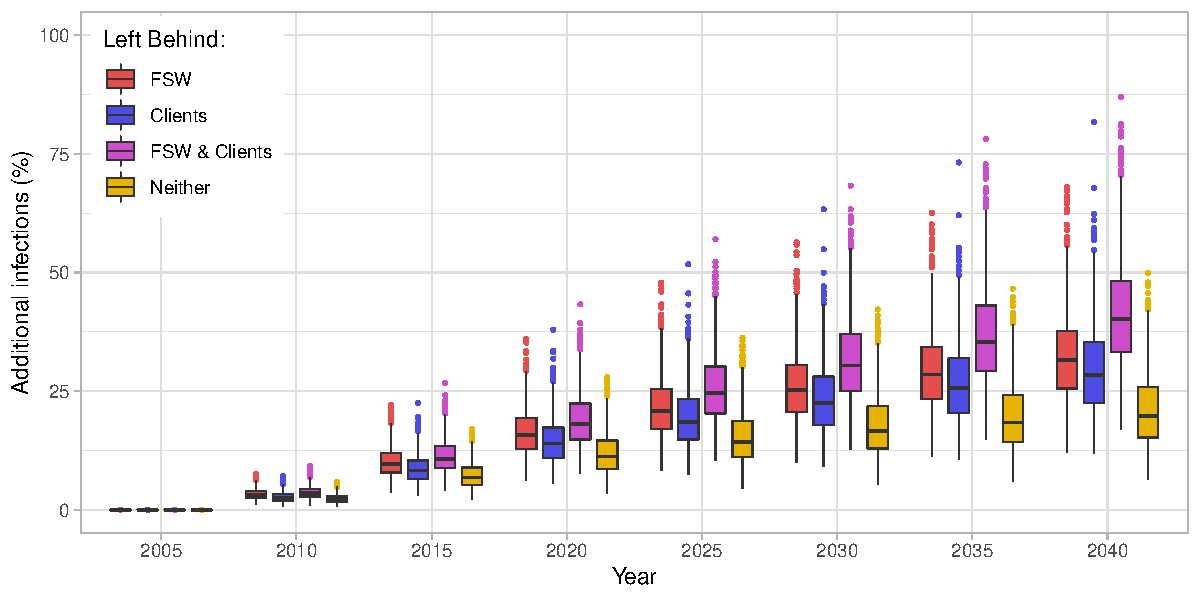
\includegraphics[width=\linewidth]{art_1_inf_add}
  \caption{Cumulative additional HIV infections (\%) in counterfactual scenarios (\casmid overall by 2020)
    vs the base case scenario (\cashigh by 2020).
    Scenarios explore reduced cascades (\caslow by 2020) among FSW, clients of FSW, both, or neither
    as part of reduced cascade overall.}
  \label{fig:obj.1.inf.add}
\end{figure}
%===================================================================================================
\subsection{Conditions under which cascade differences matter most}\label{res.obj.2}
* under construction * \begingroup\color{lightgray}
Figure~\ref{fig:obj.2.inf} illustrates the standardized effects of
disproportionate viral unsuppression among FSW and clients versus the population overall ($d$)
on cumulative additional infections versus the base case by 2040,
controlling for population-overall unsuppression (effect not shown).
Trends were consistent across multiple time horizons (Figure~\ref{fig:obj.2.inf.t})
and for additional incidence in 2030 (Figure~\ref{fig:obj.2.inc}).
However, when stratifying cumulative additional infections by sub-population
(FSW, clients, and everybody else),
some effect trends differed (Figure~\ref{fig:obj.2.inf.pop}).
% For the same population-overall viral suppression,
Consistent with Objective~\ref{obj:1} results,
disproportionate viral unsuppression among FSW and clients versus the population overall
was associated with more additional infections.
\par
Disproportionate unsuppression among FSW was associated with more infections in the context of:
larger FSW and client population sizes; and
larger HIV prevalence ratio among FSW versus lower risk women; and
larger HIV prevalence ratio among clients versus lower risk men.
Disproportionate unsuppression among clients was associated with more infections in the context of:
larger client population size;
larger HIV prevalence ratio among among clients versus lower risk men;
smaller HIV prevalence ratio among FSW versus lower risk women; and
shorter duration buying sex.
\endgroup
\begin{figure}
  \begingroup\color{lightgray}
  \includegraphics[draft,width=\linewidth]{example-image-a}%{art_2_inf}
  \caption{Partial rank correlation coefficients reduced viral suppression (d) among FSW and clients
    on cumulative additional infections by 2040,
    plus effect modification by epidemic conditions,
    controlling for population-overall viral suppression}
  \label{fig:obj.2.inf}
  \floatfoot{
    Points and lines show the mean and 95\% confidence interval for $\beta$ terms from Eq.~(\ref{eq:obj.2}).
    d\,X: absolute difference in viral suppression among group X versus the population overall;
    FSW: female sex workers;
    Clients: of FSW;
    LR: lower risk;
    Duration: average time spent in the risk group;
    \% Pop: relative population size;
    HIV PR: HIV prevalence ratio.
    All model variables were standardized like
    $\hat{x}_k = (x_k - \mu_{x_k}) / \sigma_{x_k}$
    to reflect the relative influence of variables.}
  \endgroup
\end{figure}
\par